\documentclass{article}

\usepackage[margin=1in]{geometry}

\usepackage{lmodern}
\usepackage{amsmath}
\usepackage{amssymb}
\usepackage{upgreek}
\usepackage{pgfplots}
\usepackage[normalem]{ulem}

\pgfplotsset{compat=1.11}
\usetikzlibrary{decorations.markings}
\usepgfplotslibrary{polar}


\begin{document}

\section{Curvas Parametrizadas}
De modo geral, podemos descrever uma curva plana por uma \uline{parametriza\c{c}\~ao}:
\[ \vec{r}(t) = (x(t), y(t)) \qquad \text{onde $x(t)$ e $y(t)$ s\~ao fun\c{c}\~oes da vari\'avel $t$.} \]
Exemplo: \\[-5pt]

$y = 2x \quad \rightarrow \quad \vec{r}(t) = (t, 2t)$

\subsection{Vetor Tangente}
O vetor \uline{tangente} \`a curva $\vec{r}(t) = (x(t),\, y(t))$ em um ponto $(x(t_\uplambda),\, y(t_\uplambda))$ \'e:
\[ \vec{v}(t_\uplambda) = \vec{x}\,'(t_\uplambda)\vec{\dot{\imath}} \> + \> \vec{y}\,'(t_\uplambda)\vec{\dot{\jmath}} \]
Denota-se $\vec{r}\,'(t_\uplambda)$. \\[5pt]
Exemplo:

Vetor tangente \`a curva $\vec{r}(t) = (t,\, 2t)$ no ponto $(3, 6)$:
\begin{gather*}
  (3, 6) \>\Rightarrow\> t_\uplambda = 3 \\[5pt]
  \vec{x}\,'(t) = 1 \\
  \vec{y}\,'(t) = 2 \\
  \therefore \\
  \vec{v}\,'(3) = \vec{\dot{\imath}} + 2\vec{\dot{\jmath}}
\end{gather*}
O respectivo vale para curvas no espa\c{c}o.

\subsection{Gr\'aficos}

\begin{tabular}{cc}
  $\vec{r}(t) = (\cos t, 0, \sin t)$ & $\vec{r}(t) = (\cos t, \sin t, t)$ \\[5pt]
  \vtop{\null\hbox{
    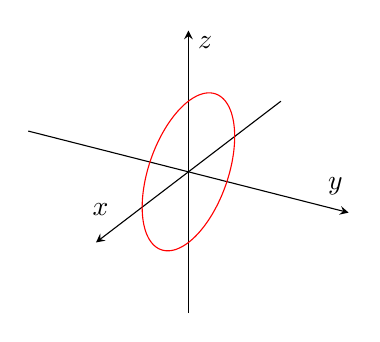
\begin{tikzpicture}
      \begin{axis}[
          view       = {120}{30},
          axis lines = middle,
          xlabel     = $x$,
          ylabel     = $y$,
          zlabel     = $z$,
          zmax       = 2,
          zmin       = -2,
          xmax       = 2,
          xmin       = -2,
          height     = 8cm,
          width      = 8cm,
          xtick      = \empty,
          ytick      = \empty,
          ztick      = \empty
        ]
        \addplot3+ [
          domain    = 0:2*pi,
          samples   = 400,
          samples y = 0,
          mark      = none,
          red,
        ]
        ( {cos(deg(x))}, {0}, {sin(deg(x))} );
      \end{axis}
    \end{tikzpicture}
  }}
  &
  \qquad\vtop{\null\hbox{
    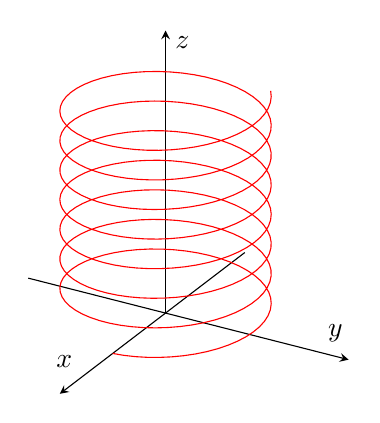
\begin{tikzpicture}
      \begin{axis}[
          view       = {120}{30},
          axis lines = middle,
          xlabel     = $x$,
          ylabel     = $y$,
          zlabel     = $z$,
          zmax       = 60,
          xmax       = 2,
          xmin       = -1.5,
          ymax       = 2,
          ymin       = -1.5,
          height     = 8cm,
          width      = 8cm,
          xtick      = \empty,
          ytick      = \empty,
          ztick      = \empty
        ]
        \addplot3+ [
          domain     = 0:14.7*pi,
          samples    = 400,
          samples y  = 0,
          mark       = none,
          red,
        ]
        ( {cos(deg(x))},{sin(deg(x))},{x});
      \end{axis}
    \end{tikzpicture}
  }}
\end{tabular}


\pagebreak
\subsection{Comprimento de Curvas}
O comprimento de uma curva $\boldsymbol{\gamma}(t)$ no plano \'e dado por
\begin{align*}
  l(\boldsymbol{\gamma}(t)) \quad &= \quad
  \lim_{\Delta t \to 0} { \sum_i \sqrt{ {\left(\frac{x(t_{i+1}) - x(t_i)}{\Delta t}\right)}^2 + { \left(\frac {y(t_{i+1}) - y(t_i)}{\Delta t}\right) }^2 } \cdot \Delta t } \\
  &= \quad \int\limits_a^b \sqrt{{(x'(t))}^2 + {(y'(t))}^2} \cdot dt
\end{align*}
Para uma curva $\boldsymbol{\gamma}(t)$ no espa\c{c}o, analogamente:
\[ l(\boldsymbol{\gamma}(t)) = \int\limits_a^b \sqrt{{(x'(t))}^2 + {(y'(t))}^2 + {(z'(t))}^2} \cdot dt \]
Exemplo:
\begin{figure}[!h]
  \qquad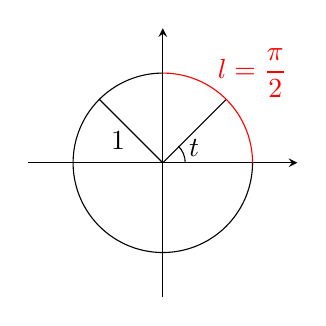
\begin{tikzpicture}
    \begin{axis}[
        axis lines = center,
        xmax       = 1.5,
        xmin       = -1.5,
        ymax       = 1.5,
        ymin       = -1.5,
        height     = 5cm,
        width      = 5cm,
        xtick      = \empty,
        ytick      = \empty,
        black
      ]
      \addplot [
        domain=pi/2:2*pi,
        samples=150,
        black
      ] ({cos(deg(x))}, {sin(deg(x))});
      \addplot [
        domain = -sqrt(2)/2 : sqrt(2)/2,
        samples = 100,
        black
      ] {abs(x)};
      \addplot [
        domain=0:pi/2,
        samples= 50,
        red
      ] ({cos(deg(x))}, {sin(deg(x))});
      
      \node at (-0.5, 0.25) {$1$};
      
      \draw (axis cs:.25,0) arc [radius=.3cm,start angle=0,end angle=45];
      \node at (0.35, 0.17) {$t$};
      
      \node [red] at (1, 1) {$l = \dfrac{\pi}{2}$};
    \end{axis}
  \end{tikzpicture}
\end{figure}

$\boldsymbol{\gamma}(t) = (\cos t, \sin t)$ \\[-5pt]

Obtemos o arco acima variando $t$ entre $a = 0$ e $b = \dfrac{\pi}{2}$. \\[-5pt]

Logo
\begin{align*}
  l &= \int\limits_0^{\pi/2} \sqrt{ {(-\sin t)}^2 + {(\cos t)}^2 } \cdot dt \\
  &= \int\limits_0^{\pi/2} 1 \cdot dt \\[1pt]
  &= \frac{\pi}{2}
\end{align*}



\pagebreak
\section{Coordenadas Polares}
Um ponto em coordenadas polares \'e definido por um raio e um \^angulo:
\[ p = {(r, \theta)}_{polar} \]

\begin{tabbing}
  Exemplo: \= Se $p = {\left(5, \frac{\pi}{4}\right)}_{polar}$ \\
  \>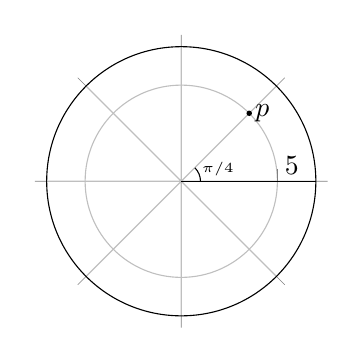
\begin{tikzpicture}
    \begin{polaraxis} [
        ymax = 7,
        height = 5cm,
        width  = 5cm,
        ytick={5},
        xticklabel = \empty,
        yticklabel = \empty,
      ]
      \node [circle,fill,inner sep=.7pt] at (45, 5) {};
      \node at (40, 5.5) {$p$};
      \draw (axis cs:0,1) arc [radius=.24cm,start angle=0,end angle=45];
      
      \node at (18, 2) {\tiny $\pi/4$};
      \node at (8, 5.8) {$5$};
    \end{polaraxis}
  \end{tikzpicture}
\end{tabbing}
\underline{Conven\c{c}\~oes}:
\begin{itemize}
  \item $\theta > 0$ se medido, a partir do eixo polar, no sentido anti-hor\'ario.
  \item $\theta < 0$ se medido, a partir do eixo polar, no sentido hor\'ario.
  \item ${(-r, \theta)}_{polar} = {(r, \theta - \pi)}_{polar}$ \\ [5pt]
    Exemplo: $(-3, \dfrac{\pi}{4}) = (3, \dfrac{5\pi}{4})$ \\
    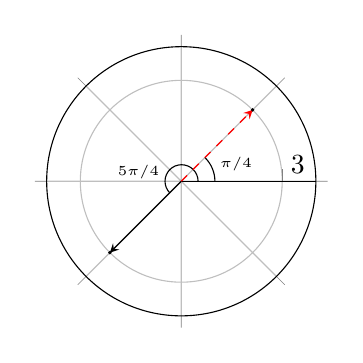
\begin{tikzpicture}
    \begin{polaraxis} [
        ymax = 4,
        height = 5cm,
        width  = 5cm,
        ytick={3},
        xticklabel = \empty,
        yticklabel = \empty,
      ]
      \draw [>=stealth,->] (0,0) -- (225, 3);
      \node [circle,fill,inner sep=.5pt] at (225, 3) {};
      \draw (axis cs:0, 0.5) arc [radius=.21cm,start angle=0,end angle=225];
      \node at (168, 1.3) {\tiny $5\pi/4$};

      \draw [>=stealth,->, red, dashed] (0,0) -- (45, 3);
      \node [circle,fill,inner sep=.5pt] at (45, 3) {};
      \draw (axis cs:0,1) arc [radius=.42cm,start angle=0,end angle=45];
      \node at (17, 1.7) {\tiny $\pi/4$};
      
      \node at (8, 3.5) {$3$};
    \end{polaraxis}
  \end{tikzpicture}
  \item $\forall \theta: {(0, \theta)}_{polar} = 0$
\end{itemize}

\subsection{Rela\c{c}\~ao Entre Sistemas de Coordenadas}
\begin{figure}[!h]
  \centering
  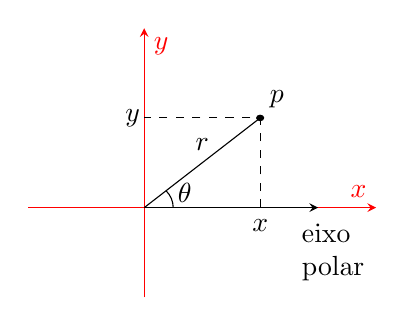
\begin{tikzpicture}
    \begin{axis}[
        axis lines = center,
        xlabel     = $x$,
        ylabel     = $y$,
        xmax       = 2,
        xmin       = -1,
        ymax       = 2,
        ymin       = -1,
        height     = 5cm,
        width      = 6cm,
        xtick      = \empty,
        ytick      = \empty,
        red
      ]
      \addplot [
        domain=0:1,
        samples=200,
        black
      ] {x};
      
      \node [black] at (0.5, 0.7) {$r$};
      
      \draw [black, dashed] (axis cs: 1, 0) |- (axis cs: 0, 1);
      \node [black] at (1, -0.2) {$x$};
      \node [black] at (-0.1, 1) {$y$};
  
      \draw [black] (axis cs:.25,0) arc [radius=.3cm,start angle=0,end angle=45];
      \node [black] at (0.35, 0.17) {$\small\theta$};
      
      \draw [>=stealth,->, black] (0,0) -- (1.5,0);
      \node [black, text width=1cm] at (1.7, -0.5) {eixo polar};
  
      \draw [black, fill=black] (1,1) circle (0.03) node[above right] {$p$};
    \end{axis}
  \end{tikzpicture}
\end{figure}
\vspace{-15pt}
\[ p = {(r,\theta)}_{polar} = {(x, y)}_{ret} \]
\begin{alignat*}{3}
  &\forall r, \theta &&: {(r, \theta)}_{polar} &&= {(r \cdot \cos \theta,\, r \cdot \sin \theta)}_{ret} \\
  &\forall x, y &&: {(x, y)}_{ret} &&= {\left(\sqrt{x^2 + y^2},\, \arctan{\frac{y}{x}}\right)}_{ret}
\end{alignat*}

\subsection{Curvas Polares}
Uma curva polar \'e definida por uma equa\c{c}\~ao entre as coordenadas polares dos pontos da curva (equa\c{c}\~ao polar). \\

\begin{tabbing}
  Exemplos: \= $r^2 + e^{r\theta} = 0$ \\[5pt]
  \> $0 \cdot \theta + r - 25 = 0 \quad\Rightarrow\quad r = 25$ \\
  \>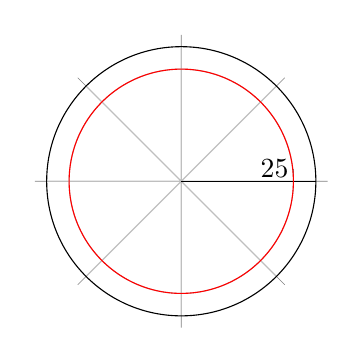
\begin{tikzpicture}
    \begin{polaraxis} [
        ymax = 30,
        height = 5cm,
        width  = 5cm,
        ytick={25},
        xticklabel = \empty,
        yticklabel = \empty,
      ]
      \addplot [
        domain=0:360,
        samples=200,
        red
      ] {25};
      
      \node at (8, 21) {$25$};
    \end{polaraxis}
  \end{tikzpicture} \\[5pt]
  \> $\theta + \frac{\pi}{6} = 0 \quad\Rightarrow\quad \theta = -\frac{\pi}{6}$ \\
  \>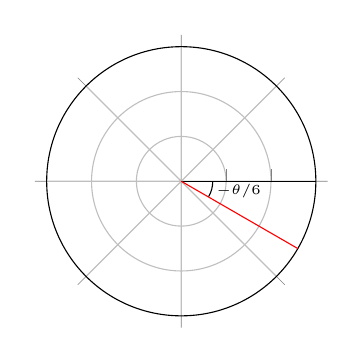
\begin{tikzpicture}
    \begin{polaraxis} [
        ymax = 3,
        height = 5cm,
        width  = 5cm,
        ytick  = {1,2},
        xticklabel = \empty,
        yticklabel = \empty,
      ]
      \addplot [
        domain=0:360,
        samples=200,
        red
      ] ({deg(-pi/6)}, {x});
      
      \draw [black] (axis cs: 331, .7) arc [radius=.38cm,start angle=330,end angle=360];
      \node at (350, 1.3) {\tiny $-\theta/6$};
    \end{polaraxis}
  \end{tikzpicture} \\[5pt]
  \> $r = \cos{(2\theta)}$ \\[5pt]
  \>\quad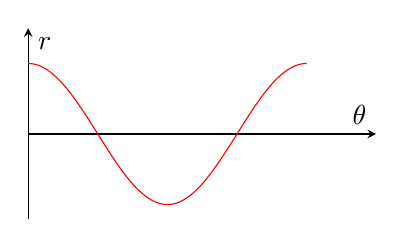
\begin{tikzpicture}
      \begin{axis}[
          axis lines = middle,
          xlabel     = $\theta$,
          ylabel     = $r$,
          xmax       = 3*pi,
          xmin       = pi/2,
          ymax       = 1.5,
          ymin       = -1.2,
          height     = 4cm,
          width      = 6cm,
          xtick      = \empty,
          ytick      = \empty,
        ]
        \addplot [
          domain=0:5*pi/2,
          samples=200,
          red
        ] {sin(deg(x))};
      \end{axis}
  \end{tikzpicture} \\
  \>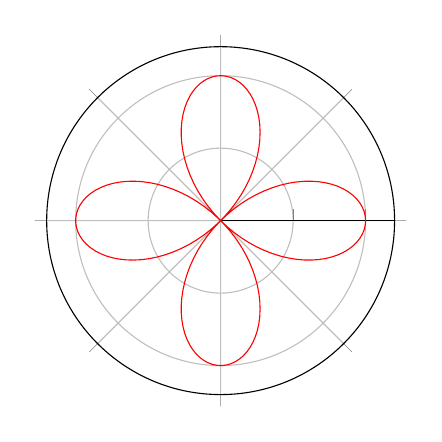
\begin{tikzpicture}
    \begin{polaraxis} [
        ymax = 1.2,
        height = 6cm,
        width  = 6cm,
        ytick  = {0.5,1},
        xticklabel = \empty,
        yticklabel = \empty,
      ]
      \addplot [
        domain=0:360,
        samples=200,
        red
      ] {cos(2*x)};
    \end{polaraxis}
  \end{tikzpicture}
\end{tabbing}



\end{document}
